\documentclass[11pt,a4paper]{article}

\usepackage[utf8]{inputenc}
\usepackage[T1]{fontenc}
\usepackage{mathpazo}
\usepackage[scaled=0.92]{helvet}
\usepackage[margin=1in]{geometry}
\usepackage{graphicx}
\usepackage{amsmath,amssymb,amsfonts}
\usepackage{booktabs}
\usepackage{tabularx}
\usepackage{setspace}
\usepackage{titlesec}
\usepackage{fancyhdr}
\usepackage{float}
\usepackage{caption}
\usepackage{microtype}
\usepackage{tikz}
\usepackage{xcolor}
\usepackage{listings}
\usepackage[hidelinks]{hyperref}

\usetikzlibrary{shapes.geometric, arrows.meta, positioning, calc, matrix, fit, backgrounds}

\setstretch{1.15}
\setlength{\parindent}{0pt}
\setlength{\parskip}{0.8em}
\sloppy

\titleformat{\section}{\normalfont\large\bfseries\sffamily}{\thesection}{1em}{}
\titleformat{\subsection}{\normalfont\normalsize\bfseries\sffamily}{\thesubsection}{1em}{}
\titleformat{\subsubsection}{\normalfont\normalsize\itshape\sffamily}{\thesubsubsection}{1em}{}

\pagestyle{fancy}
\fancyhf{}
\fancyhead[L]{\small\sffamily Tipe-Tipe Requirement}
\fancyhead[R]{\small\sffamily\thepage}
\renewcommand{\headrulewidth}{0.4pt}

\captionsetup{font=small,labelfont=bf,labelsep=period}

\renewenvironment{abstract}
{\small
	\begin{center}\textbf{\sffamily Abstrak}\end{center}
	\begin{quote}}
	{\end{quote}}

\lstdefinestyle{code}{
	basicstyle=\ttfamily\small,
	frame=single,
	rulecolor=\color{black},
	breaklines=true,
	showstringspaces=false,
	columns=fullflexible,
	keepspaces=true,
	framesep=6pt,
	aboveskip=1em,
	belowskip=1em,
	xleftmargin=0pt
}

\lstdefinestyle{out}{
	basicstyle=\ttfamily\small,
	frame=tb,
	rulecolor=\color{black},
	breaklines=true,
	showstringspaces=false,
	columns=fullflexible,
	keepspaces=true,
	framesep=4pt,
	aboveskip=1em,
	belowskip=1em
}

\title{\vspace{-1.5cm}\textbf{\sffamily\LARGE Tipe-Tipe Requirement\\ dari Business sampai Non-Functional}}
\author{
	\textbf{Muhammad Riduwan Khafidi} \\
	\small Program Studi Teknik Rekayasa Perangkat Lunak \\
	\small Politeknik Negeri Batam \\
	\small \texttt{4342611034@students.polibatam.ac.id}
}
\date{\small\today}

\begin{document}

\maketitle
\thispagestyle{empty}

\begin{abstract}
	Makalah ini membahas empat tipe requirement yang wajib dibedakan seorang analis: business, user, functional, dan non-functional. Ia tidak hanya menjelaskan definisi, tapi memberi alat uji praktis berupa diagram keputusan dan tabel perbandingan agar pembaca bisa mengklasifikasi requirement yang ditemukan di lapangan. Tujuh visualisasi dan tiga tabel menyertai pembahasan, termasuk enam dimensi pembentuk user class yang tidak selalu disebut di kelas. Sebuah studi kasus sepuluh langkah dengan sistem penjadwalan kuliah menunjukkan bagaimana keempat tipe ini saling berhubungan dan menghasilkan artefak konkret. Konsep traceability sebagai jembatan antara business need dan test case juga diperkenalkan sebagai pelengkap. Lembar rujukan cepat di akhir merangkum istilah dan template yang wajib dikuasai sebelum pertemuan kelima.
\end{abstract}

\section{Pendahuluan}

\subsection{Analogi Pembuka}

Bayangkan sebuah restoran. Di meja tamu ada menu dengan foto dan harga. Di dapur ada resep dengan takaran bahan dan urutan langkah. Di ruang manajer ada target pendapatan bulanan dan daftar supplier.

Ketiganya berbicara tentang makanan yang sama, tapi di level yang berbeda. Menu berbicara tentang \textbf{apa yang dijual}. Resep berbicara tentang \textbf{bagaimana memasaknya}. Target manajer berbicara tentang \textbf{mengapa restoran ini ada}. Kalau ketiga dokumen itu dicampur, dapur akan menerima menu sebagai instruksi masak, dan manajer akan menerima resep sebagai laporan keuangan.

Requirement juga hidup di beberapa level seperti itu. Business requirement adalah target manajer. User requirement adalah menu. System requirement adalah resep. Mencampur level-level ini adalah salah satu kesalahan paling sering dalam penulisan requirement.

\subsection{Mengapa Topik Ini Penting}

Pada minggu-minggu sebelumnya, kita mempelajari apa itu requirement, siapa stakeholder-nya, dan bagaimana analyst menjalankan perannya. Di minggu ini, kita belajar bahwa ``requirement'' bukan satu benda. Ia adalah keluarga empat tipe yang saling bergantung. Kalau salah satu tipe hilang, atau dua tipe dicampur, dokumen requirement menjadi tidak bisa diuji dan tidak bisa dilacak.

\subsection{Peta Pembahasan}

Makalah ini disusun sebagai berikut. Bagian kedua memetakan empat level requirement dalam satu hierarki. Bagian ketiga sampai keenam membahas satu per satu: business, user, functional, dan non-functional. Bagian ketujuh memberi alat uji klasifikasi. Bagian kedelapan sampai kesepuluh merangkum perbandingan, kesalahan umum, dan lembar rujukan cepat. Bagian kesebelas memandu studi kasus sepuluh langkah dengan sistem penjadwalan kuliah. Bagian kedua belas menutup dengan tiga prinsip.

\section{Peta Empat Level Requirement}

Requirement hidup di empat level. Perhatikan Gambar~\ref{fig:four-levels}. Semakin ke atas, semakin abstrak dan semakin dekat ke tujuan bisnis. Semakin ke bawah, semakin konkret dan semakin dekat ke kode.

\begin{figure}[H]
	\centering
	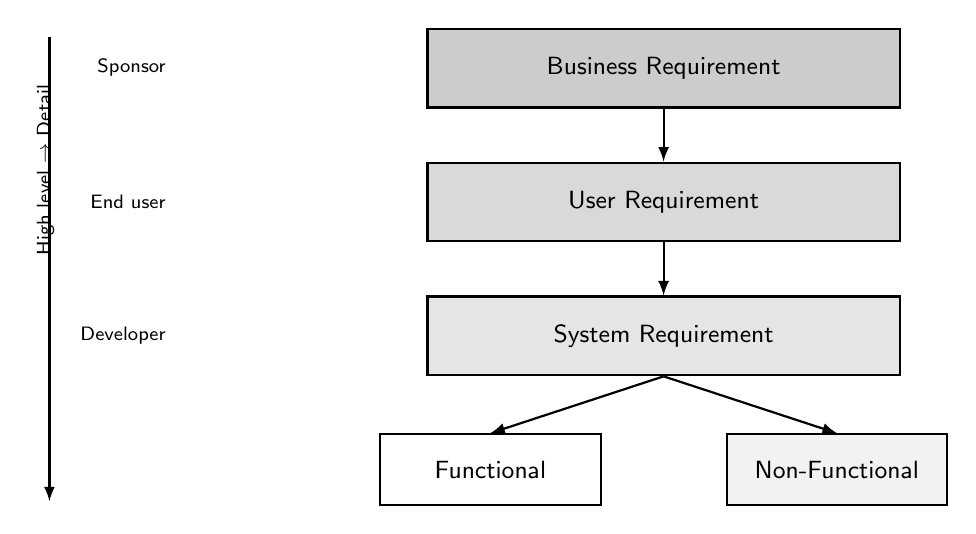
\begin{tikzpicture}[
			lvlbox/.style={rectangle, draw=black, thick, minimum width=6cm, minimum height=1.0cm, align=center, font=\sffamily\small},
			leafbox/.style={rectangle, draw=black, thick, minimum width=2.8cm, minimum height=0.9cm, align=center, font=\sffamily\small},
			arr/.style={draw, thick, -latex},
			side/.style={font=\sffamily\scriptsize, anchor=east}
		]
		\node[lvlbox, fill=black!20] (biz) at (0, 5.0) {Business Requirement};
		\node[lvlbox, fill=black!15] (usr) at (0, 3.3) {User Requirement};
		\node[lvlbox, fill=black!10] (sys) at (0, 1.6) {System Requirement};

		\node[leafbox, fill=white]   (fn)  at (-2.2, -0.1) {Functional};
		\node[leafbox, fill=black!5] (nfr) at ( 2.2, -0.1) {Non-Functional};

		\draw[arr] (biz.south) -- (usr.north);
		\draw[arr] (usr.south) -- (sys.north);
		\draw[arr] (sys.south) -- (fn.north);
		\draw[arr] (sys.south) -- (nfr.north);

		\node[side] at (-6.2, 5.0) {Sponsor};
		\node[side] at (-6.2, 3.3) {End user};
		\node[side] at (-6.2, 1.6) {Developer};

		\draw[thick, -latex] (-7.8, 5.4) -- (-7.8, -0.5);
		\node[font=\sffamily\scriptsize, anchor=west, rotate=90] at (-7.85, 2.5) {High level $\to$ Detail};
	\end{tikzpicture}
	\caption{Empat level requirement dan siapa yang membacanya.}
	\label{fig:four-levels}
\end{figure}

Tiga hal yang perlu diperhatikan dari hierarki ini.

\textbf{Pertama, setiap level punya pembaca utama yang berbeda.} Business requirement dibaca sponsor. User requirement dibaca end user. System requirement dibaca developer. Menulis business requirement dalam bahasa developer adalah kesalahan yang setara dengan menulis menu restoran dalam bahasa koki.

\textbf{Kedua, setiap level harus bisa dilacak ke level di atasnya.} Setiap functional requirement wajib bisa dilacak balik ke satu user requirement, dan user requirement wajib bisa dilacak balik ke satu business requirement. Kalau tidak, requirement itu tidak punya alasan untuk ada.

\textbf{Ketiga, system requirement adalah satu-satunya yang dipecah dua.} Business dan user requirement cukup satu lapis. System requirement harus dipecah menjadi functional dan non-functional, karena keduanya diuji dengan cara yang berbeda.

Pelacakan antar level ini disebut \textbf{traceability}. Ia tidak selalu eksplisit di slide, tapi tanpa traceability, dokumen requirement hanya tumpukan kalimat.

\section{Business Requirement}

Business requirement menjelaskan \textbf{mengapa} organisasi melakukan proyek ini. Apa yang bisnis coba capai dengan proyek ini. Ia mencakup visi dan scope proyek, dan biasanya dinyatakan dalam project charter, business case, atau vision and scope statement.

Business requirement dikumpulkan dari project owner, stakeholder, dan tim proyek. Tujuannya satu: menyusun tujuan tingkat tinggi proyek. Tanpa informasi ini, tim tidak akan tahu mengapa mereka membangun sesuatu.

Tapi perlu dicatat: \textbf{kita tidak bisa membangun software hanya dari informasi tingkat tinggi ini}. Business requirement adalah arah, bukan rencana. Ia memberi tahu kita ke mana harus pergi, bukan jalan mana yang harus diambil.

Ada tujuh dokumen yang biasa dipakai untuk mengomunikasikan business requirement: problem statement, project vision, project constraints (budget, schedule, resources), project objectives, project scope statements, business process analysis, dan stakeholder analysis.

Yang paling sering dilupakan adalah \textbf{business process analysis}. Tujuannya menentukan bagaimana proses bisnis akan berjalan. Sebelum mengotomasi proses, kita wajib memahaminya dulu. Perhatikan Gambar~\ref{fig:process-bike}.

\begin{figure}[H]
	\centering
	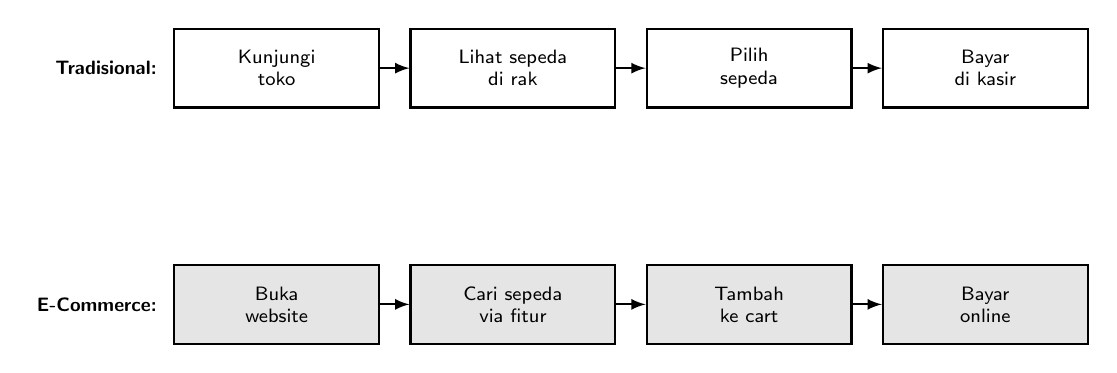
\begin{tikzpicture}[
			procbox/.style={rectangle, draw=black, thick, minimum width=2.6cm, minimum height=1.0cm, align=center, font=\sffamily\scriptsize, inner sep=3pt},
			arr/.style={draw, thick, -latex},
			rowlabel/.style={font=\sffamily\scriptsize\bfseries, anchor=east}
		]
		\node[rowlabel] at (-1.4, 1.5) {Tradisional:};
		\node[procbox, fill=white] (t1) at (0, 1.5) {Kunjungi\\toko};
		\node[procbox, fill=white] (t2) at (3, 1.5) {Lihat sepeda\\di rak};
		\node[procbox, fill=white] (t3) at (6, 1.5) {Pilih\\sepeda};
		\node[procbox, fill=white] (t4) at (9, 1.5) {Bayar\\di kasir};
		\draw[arr] (t1) -- (t2);
		\draw[arr] (t2) -- (t3);
		\draw[arr] (t3) -- (t4);

		\node[rowlabel] at (-1.4, -1.5) {E-Commerce:};
		\node[procbox, fill=black!10] (e1) at (0, -1.5) {Buka\\website};
		\node[procbox, fill=black!10] (e2) at (3, -1.5) {Cari sepeda\\via fitur};
		\node[procbox, fill=black!10] (e3) at (6, -1.5) {Tambah\\ke cart};
		\node[procbox, fill=black!10] (e4) at (9, -1.5) {Bayar\\online};
		\draw[arr] (e1) -- (e2);
		\draw[arr] (e2) -- (e3);
		\draw[arr] (e3) -- (e4);
	\end{tikzpicture}
	\caption{Business process tradisional dan versi otomasi untuk pembelian sepeda.}
	\label{fig:process-bike}
\end{figure}

Perhatikan bahwa alur e-commerce bukan sekadar alur tradisional yang dipindahkan ke layar. Setiap langkah berubah maknanya. ``Kunjungi toko'' menjadi ``buka website''. ``Lihat sepeda di rak'' menjadi ``cari sepeda via fitur pencarian''. ``Bayar di kasir'' menjadi ``bayar online''. Bisnis proses yang tidak dipahami sebelum diotomasi akan menghasilkan sistem yang memaksa user bekerja dengan cara mesin, bukan sebaliknya.

\section{User Requirement}

User requirement menguraikan apa saja yang bisa dilakukan user dengan produk, dan mendefinisikan apa yang produk harus lakukan untuk user. User adalah individu yang akan memakai software kita. Mereka sering disebut end user.

End user sangat kritis bagi keberhasilan produk. Itulah sebabnya user requirement adalah salah satu requirement paling penting. Bentuknya bisa use case, user story, atau scenario.

\subsection{Enam Dimensi User Class}

Tidak semua user sama. Menganggap semua user identik adalah kesalahan yang menghasilkan produk yang tidak nyaman untuk siapa pun. User bisa dikelompokkan menjadi beberapa user class berdasarkan enam dimensi. Perhatikan Gambar~\ref{fig:six-dimensions}.

\begin{figure}[H]
	\centering
	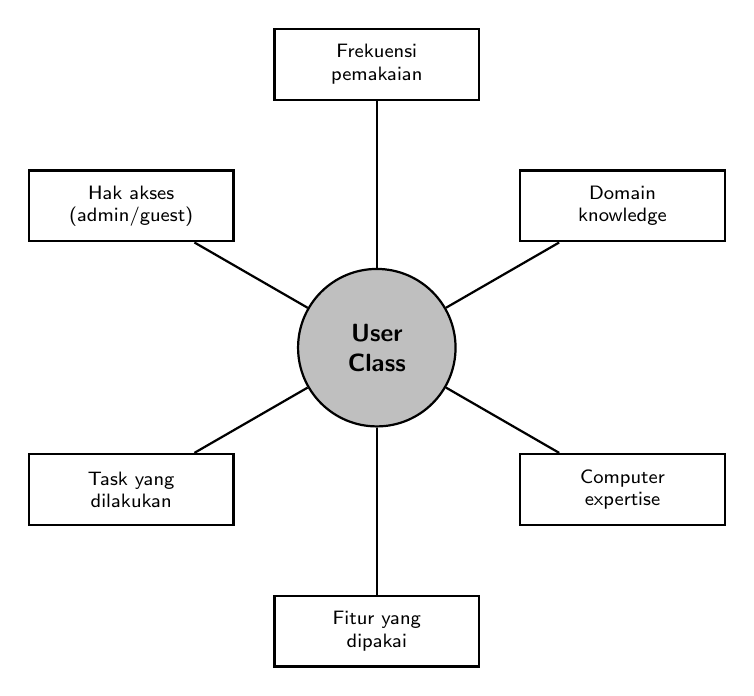
\begin{tikzpicture}[
			hub/.style={circle, draw=black, thick, fill=black!25, minimum size=2cm, align=center, font=\sffamily\small\bfseries},
			dimbox/.style={rectangle, draw=black, thick, fill=white, minimum width=2.6cm, minimum height=0.9cm, align=center, font=\sffamily\scriptsize, inner sep=3pt},
			arr/.style={draw, thick}
		]
		\node[hub] (c) at (0,0) {User\\Class};

		\node[dimbox] (d1) at (0,     3.6) {Frekuensi\\pemakaian};
		\node[dimbox] (d2) at (3.12,  1.8) {Domain\\knowledge};
		\node[dimbox] (d3) at (3.12, -1.8) {Computer\\expertise};
		\node[dimbox] (d4) at (0,    -3.6) {Fitur yang\\dipakai};
		\node[dimbox] (d5) at (-3.12,-1.8) {Task yang\\dilakukan};
		\node[dimbox] (d6) at (-3.12, 1.8) {Hak akses\\(admin/guest)};

		\draw[arr] (c) -- (d1);
		\draw[arr] (c) -- (d2);
		\draw[arr] (c) -- (d3);
		\draw[arr] (c) -- (d4);
		\draw[arr] (c) -- (d5);
		\draw[arr] (c) -- (d6);
	\end{tikzpicture}
	\caption{Enam dimensi yang membedakan user class.}
	\label{fig:six-dimensions}
\end{figure}

Setelah mengelompokkan user ke dalam kelas, kita bisa menandai beberapa kelas sebagai \textbf{favored}. Favored user class adalah kelas yang paling kritis bagi keberhasilan produk atau bisnis. Mereka bukan yang paling banyak jumlahnya, tapi yang paling menentukan apakah produk ini berhasil atau tidak.

Contoh nyata ada di sistem chemical tracking. Chemist (sekitar 1000 orang) memakai sistem beberapa kali sehari untuk meminta bahan kimia dari vendor dan gudang. Health and Safety Department Staff memakai sistem hanya sekali per kuartal untuk menghasilkan laporan kepatuhan. Buyers (sekitar 5 orang) memproses permintaan kimia yang diajukan pihak lain. Chemical Stockroom Staff (6 teknisi dan 1 supervisor) mengelola inventori dan memproses permintaan chemist.

Kalau kita melihat dari frekuensi pemakaian, Chemist adalah yang paling sering. Tapi dari dampak regulasi, Health and Safety Staff justru yang paling kritis. Keduanya bisa ditandai favored, meskipun alasan favored-nya berbeda.

\subsection{Sumber User Requirement}

Ada tujuh sumber yang bisa dipakai untuk menggali user requirement:

\textbf{Pertama, wawancara dan diskusi dengan potential users.} Ini sumber paling langsung, tapi juga paling memakan waktu.

\textbf{Kedua, dokumen yang mendeskripsikan produk saat ini atau kompetitor.} Berguna untuk memahami standar industri.

\textbf{Ketiga, problem report dan enhancement request dari sistem yang sedang berjalan.} Ini sumber paling jujur karena berasal dari keluhan nyata.

\textbf{Keempat, analisis event dan respons dari sistem.} Berguna untuk sistem yang sudah berjalan dan punya log.

\textbf{Kelima, marketing survey dan kuesioner.} Cocok untuk mengukur preferensi user dalam jumlah besar.

\textbf{Keenam, observasi langsung terhadap user yang bekerja.} Cara terbaik menemukan kebutuhan yang tidak pernah diucapkan user karena dianggap remeh.

\textbf{Ketujuh, scenario analysis terhadap task user.} Berguna untuk memetakan alur kerja yang kompleks.

\subsection{Product Champion}

Product Champion adalah beberapa member key atau influential dari user community yang merepresentasikan user dan memberi requirement. Ia menjadi interface utama antara user dari satu user class dan requirement analyst proyek. Perhatikan Gambar~\ref{fig:champion}.

\begin{figure}[H]
	\centering
	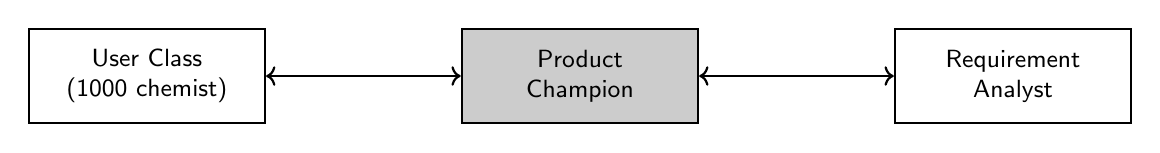
\begin{tikzpicture}[
			pcbox/.style={rectangle, draw=black, thick, minimum width=3cm, minimum height=1.2cm, align=center, font=\sffamily\small, inner sep=4pt},
			arr/.style={draw, thick, <->}
		]
		\node[pcbox, fill=white]    (users) at (-5.5, 0) {User Class\\(1000 chemist)};
		\node[pcbox, fill=black!20] (pc)    at ( 0, 0)   {Product\\Champion};
		\node[pcbox, fill=white]    (ana)   at ( 5.5, 0) {Requirement\\Analyst};

		\draw[arr] (users.east) -- (pc.west);
		\draw[arr] (pc.east)    -- (ana.west);
	\end{tikzpicture}
	\caption{Product champion sebagai interface antara user class dan analyst.}
	\label{fig:champion}
\end{figure}

Dua aturan penting tentang product champion.

\textbf{Pertama, harus real user, bukan surrogate.} Ia tidak boleh manajer yang mewakili user, atau staf pemasaran yang mengaku paham user. Ia harus benar-benar orang yang memakai sistem sehari-hari.

\textbf{Kedua, harus satu per user class.} Setiap user class punya perilaku dan kebutuhan berbeda. Product champion dari chemist tidak bisa mewakili buyers, meskipun keduanya bekerja di perusahaan yang sama.

Alasan kedua aturan ini sederhana: kalau champion-nya bukan user asli, ia akan menyampaikan apa yang \textit{ia pikir} user butuhkan, bukan apa yang \textbf{user benar-benar} butuhkan. Perbedaan kecil ini, kalau dibiarkan sampai tahap implementasi, akan menghasilkan sistem yang secara teknis berjalan tapi secara praktis tidak terpakai.

\section{System Requirement: Functional}

Functional requirement adalah perilaku yang harus produk lakukan atau dukung. Requirement ini dipakai tim pengembangan untuk membangun perilaku sistem. Biasanya dinyatakan dengan input, output, dan deskripsi perilaku itu sendiri. Perhatikan Gambar~\ref{fig:fn-io}.

\begin{figure}[H]
	\centering
	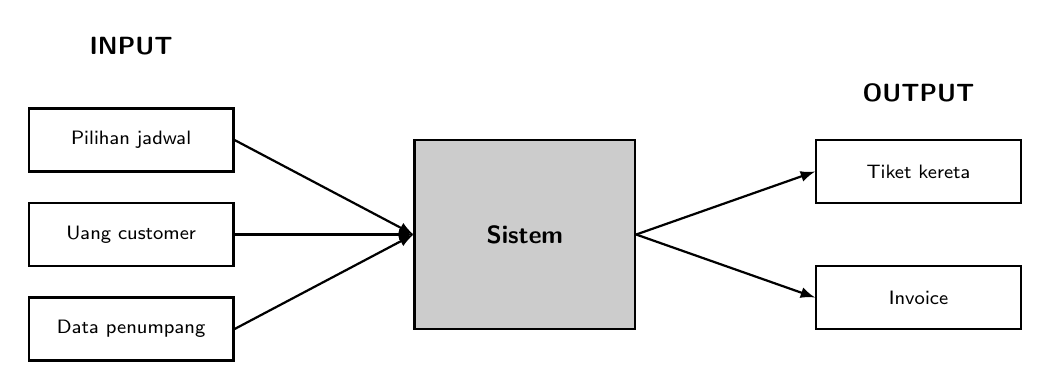
\begin{tikzpicture}[
			sysbox/.style={rectangle, draw=black, thick, fill=black!20, minimum width=2.8cm, minimum height=2.4cm, align=center, font=\sffamily\small\bfseries},
			iobox/.style={rectangle, draw=black, thick, fill=white, minimum width=2.6cm, minimum height=0.8cm, align=center, font=\sffamily\scriptsize, inner sep=3pt},
			arr/.style={draw, thick, -latex},
			tag/.style={font=\sffamily\small\bfseries}
		]
		\node[sysbox] (sys) at (0, 0) {Sistem};

		\node[iobox] (i1) at (-5, 1.2) {Pilihan jadwal};
		\node[iobox] (i2) at (-5, 0)   {Uang customer};
		\node[iobox] (i3) at (-5, -1.2){Data penumpang};

		\node[iobox] (o1) at (5, 0.8)  {Tiket kereta};
		\node[iobox] (o2) at (5, -0.8) {Invoice};

		\draw[arr] (i1.east) -- (sys.west);
		\draw[arr] (i2.east) -- (sys.west);
		\draw[arr] (i3.east) -- (sys.west);
		\draw[arr] (sys.east) -- (o1.west);
		\draw[arr] (sys.east) -- (o2.west);

		\node[tag] at (-5, 2.4) {INPUT};
		\node[tag] at ( 5, 1.8) {OUTPUT};
	\end{tikzpicture}
	\caption{Struktur khas functional requirement: input, proses, output.}
	\label{fig:fn-io}
\end{figure}

Contoh-contoh functional requirement yang sering muncul:

\textbf{Contoh sistem,} ``Sistem menampilkan nama, ukuran total, ruang tersedia, dan format dari flash drive yang terhubung ke port USB.''

\textbf{Contoh singkat,} ``Tambahkan customer.'' ``Cetak invoice.''

\textbf{Contoh dari produk fisik,} kalau kita memandang karton susu sebagai sistem, functional requirement-nya adalah ``kemampuan menampung cairan tanpa bocor.''

Yang membedakan functional requirement dari yang lain adalah: ia bisa diuji dengan skenario konkret. Kalau kita tidak bisa membayangkan cara mengujinya dengan data nyata, kalimat itu bukan functional requirement, mungkin masih user requirement atau bahkan business requirement.

\section{System Requirement: Non-Functional}

Non-functional requirement mendeskripsikan \textbf{seberapa baik} produk harus tampil. Ia menyentuh faktor kualitas produk. Kadang disebut quality requirements. Perhatikan Gambar~\ref{fig:fn-vs-nfr}.

\begin{figure}[H]
	\centering
	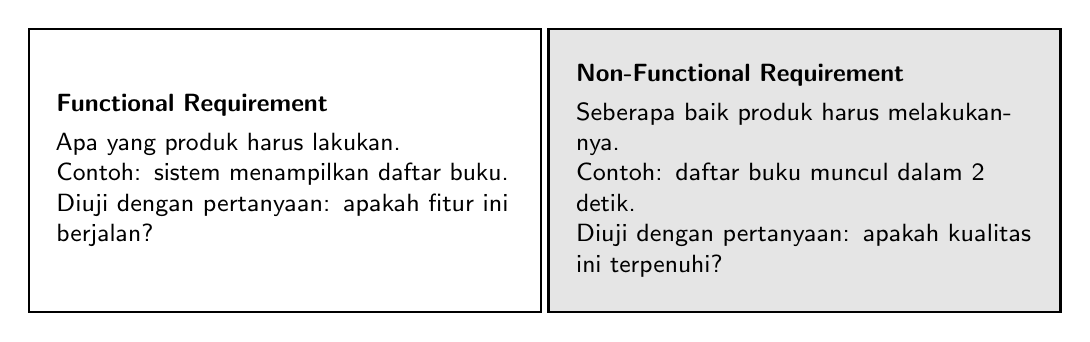
\begin{tikzpicture}[
			cmpbox/.style={rectangle, draw=black, thick, text width=5.8cm, align=left, font=\sffamily\small, inner sep=10pt, minimum height=3.6cm}
		]
		\node[cmpbox, fill=white, anchor=north west] (a) at (-6.2, 0) {
			\textbf{Functional Requirement} \\[3pt]
			Apa yang produk harus lakukan. \\
			Contoh: sistem menampilkan daftar buku. \\
			Diuji dengan pertanyaan: apakah fitur ini berjalan?
		};
		\node[cmpbox, fill=black!10, anchor=north west] (b) at (0.4, 0) {
			\textbf{Non-Functional Requirement} \\[3pt]
			Seberapa baik produk harus melakukannya. \\
			Contoh: daftar buku muncul dalam 2 detik. \\
			Diuji dengan pertanyaan: apakah kualitas ini terpenuhi?
		};
	\end{tikzpicture}
	\caption{Perbedaan cara pandang functional dan non-functional requirement.}
	\label{fig:fn-vs-nfr}
\end{figure}

Kategori non-functional requirement yang lazim meliputi: performance (response time, throughput, utilization, static volumetric), scalability, maintainability, availability, security, reliability, manageability, recoverability, dan environmental.

Contoh klasik dari slide: helm proyek (hard hat) punya non-functional requirement ``tidak boleh pecah pada tekanan kurang dari 10.000 PSI.'' Contoh ini memperjelas bahwa non-functional selalu bisa diukur dengan angka atau kriteria yang bisa diverifikasi.

Yang perlu dihindari adalah non-functional requirement yang tidak terukur, seperti ``sistem harus cepat'', ``sistem harus aman'', ``sistem harus mudah digunakan''. Tiga kalimat itu bukan requirement, melainkan harapan. Ubah menjadi ``response time kurang dari 2 detik pada 95 persen request'', ``password disimpan dengan hash bcrypt'', ``user bisa menyelesaikan task utama dalam 3 klik atau kurang''.

\section{Alat Uji Klasifikasi}

Saat menemukan satu kalimat di lapangan, kita kadang bingung: ini functional atau non-functional? Perhatikan Gambar~\ref{fig:decision}.

\begin{figure}[H]
	\centering
	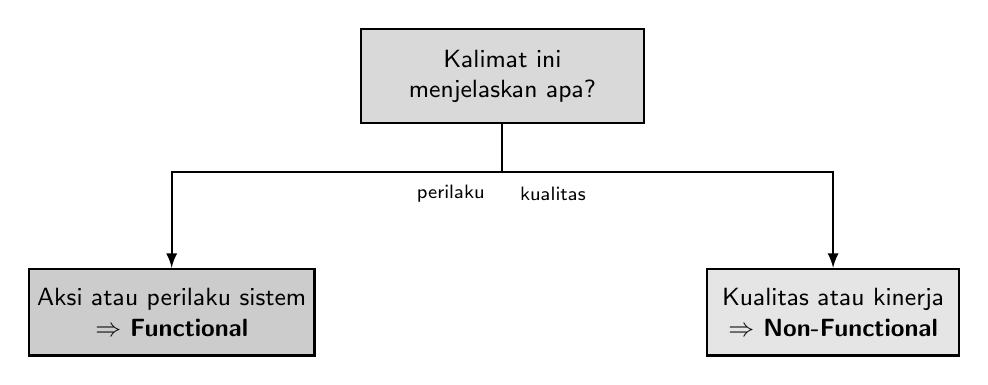
\begin{tikzpicture}[
			qnode/.style={rectangle, draw=black, thick, fill=black!15, minimum width=3.6cm, minimum height=1.2cm, align=center, font=\sffamily\small, inner sep=4pt},
			anode/.style={rectangle, draw=black, thick, fill=white, minimum width=3.2cm, minimum height=1.1cm, align=center, font=\sffamily\small, inner sep=3pt},
			arr/.style={draw, thick, -latex},
			lbl/.style={font=\sffamily\scriptsize}
		]
		\node[qnode] (root) at (0, 3) {Kalimat ini\\menjelaskan apa?};

		\node[anode, fill=black!20] (fn)  at (-4.2, 0)  {Aksi atau perilaku sistem\\$\Rightarrow$ \textbf{Functional}};
		\node[anode, fill=black!10] (nfr) at ( 4.2, 0)  {Kualitas atau kinerja\\$\Rightarrow$ \textbf{Non-Functional}};

		\draw[arr] (root.south) -- ++(0, -0.6) -| (fn.north);
		\draw[arr] (root.south) -- ++(0, -0.6) -| (nfr.north);

		\node[lbl, anchor=east] at (-0.1, 1.5) {perilaku};
		\node[lbl, anchor=west] at ( 0.1, 1.5) {kualitas};
	\end{tikzpicture}
	\caption{Alat uji cepat untuk mengklasifikasi requirement.}
	\label{fig:decision}
\end{figure}

Aturan penggunaannya sederhana. Baca kalimat requirement yang ditemukan. Kalau ia menjelaskan \textbf{apa yang sistem harus lakukan} (misalnya ``menampilkan daftar'', ``menyimpan riwayat'', ``mengirim notifikasi''), ia adalah functional requirement. Kalau ia menjelaskan \textbf{seberapa baik sistem harus melakukannya} (misalnya ``dalam 2 detik'', ``tersedia 99 persen'', ``dengan enkripsi AES-256''), ia adalah non-functional requirement.

Kalau ragu, coba ubah kalimatnya menjadi pertanyaan uji. Functional requirement diuji dengan ``apakah fitur ini berjalan?''. Non-functional diuji dengan ``apakah angka ini tercapai?''. Kalau tidak ada satu pun pertanyaan yang bisa dijawab, kalimat itu masih terlalu kabur untuk masuk dokumen requirement.

\section{Perbandingan Ringkasan}

Tabel~\ref{tab:summary} merangkum keempat tipe requirement dalam satu pandangan.

\begin{table}[H]
	\centering
	\caption{Perbandingan empat tipe requirement.}
	\label{tab:summary}
	\footnotesize
	\begin{tabularx}{\textwidth}{l X X X}
		\toprule
		Tipe           & Dijawab untuk                & Bentuk Khas                  & Pembaca Utama     \\
		\midrule
		Business       & Mengapa proyek ini ada       & Vision, scope, business case & Sponsor           \\
		User           & Apa yang bisa user lakukan   & Use case, user story         & End user          \\
		Functional     & Apa yang sistem lakukan      & Input, proses, output        & Developer         \\
		Non-functional & Seberapa baik sistem bekerja & Angka, kriteria kualitas     & Developer, tester \\
		\bottomrule
	\end{tabularx}
\end{table}

Setelah tabel ini, satu paragraf pengingat: keempat tipe ini tidak berdiri sendiri. Setiap functional requirement harus bisa dilacak ke satu user requirement, yang pada gilirannya harus bisa dilacak ke satu business requirement. Tanpa rantai pelacakan ini, requirement kehilangan konteks dan mudah berubah tanpa alasan yang jelas.

\section{Studi Kasus: Sistem Penjadwalan Kuliah}

Bagian ini memandu sepuluh langkah untuk menghasilkan artefak minggu keempat. Kasus yang dipakai: sistem penjadwalan kuliah. Tujuannya mengotomasi proses penyusunan jadwal yang sebelumnya manual oleh staf akademik.

\subsection{Langkah 1: Tulis Business Requirement}

Sebelum apa pun, tulis mengapa proyek ini ada.

\begin{lstlisting}[style=out]
Business Requirement:

Tujuan:
Mengotomasi penyusunan jadwal kuliah agar staf
akademik tidak lagi menyusun jadwal manual yang
memakan waktu 2 minggu per semester.

Ukuran keberhasilan:
- Penyusunan jadwal selesai dalam 1 hari
- Tidak ada bentrok ruang atau dosen
- Dosen bisa menyampaikan preferensi waktu

Pembaca dokumen: Kepala Staf Akademik
\end{lstlisting}

\subsection{Langkah 2: Tulis User Requirement}

Setelah business requirement, tulis apa yang tiap user class harus bisa lakukan.

\begin{lstlisting}[style=out]
User Requirement:

Staf Akademik (favored):
- Bisa mengunggah daftar mata kuliah dan dosen
- Bisa menekan tombol "Generate Jadwal"
- Bisa mengunduh jadwal dalam format PDF

Dosen (supporting):
- Bisa mengisi preferensi waktu mengajar
- Bisa melihat jadwal hasil generate

Mahasiswa (supporting):
- Bisa melihat jadwal di halaman publik
- Bisa memfilter jadwal berdasarkan semester

Pembaca dokumen: Product Champion setiap user class
\end{lstlisting}

\subsection{Langkah 3: Analisis Business Process}

Sebelum mengotomasi, petakan proses yang sedang berjalan.

\begin{lstlisting}[style=out]
Proses Tradisional (sebelum sistem):
1. Staf akademik meminta ketersediaan dosen
2. Staf mencatat preferensi dosen di Excel
3. Staf memeriksa ketersediaan ruang manual
4. Staf menyusun jadwal di Excel
5. Staf memeriksa bentrok satu per satu
6. Jika bentrok, ulangi dari langkah 3
7. Staf menerbitkan jadwal di papan pengumuman

Masalah:
- Langkah 5 bisa memakan 2 minggu
- Bentrok sering terlewat karena human error
- Revisi harus mengulang seluruh proses

Proses Otomasi (setelah sistem):
1. Staf mengunggah daftar mata kuliah dan dosen
2. Sistem menerima preferensi dosen via form
3. Sistem memeriksa bentrok otomatis
4. Sistem menghasilkan jadwal optimal
5. Staf meninjau hasil, klik "Publish"
6. Sistem menerbitkan jadwal di halaman publik
\end{lstlisting}

\subsection{Langkah 4: Identifikasi Sumber User Requirement}

Dari tujuh sumber yang ada, pilih minimal tiga.

\begin{lstlisting}[style=out]
Sumber User Requirement yang Dipakai:

1. Wawancara dengan Kepala Staf Akademik (90 menit)
   Topik: kendala penyusunan manual, harapan sistem

2. Wawancara dengan 5 dosen (masing-masing 20 menit)
   Topik: preferensi waktu, konflik yang sering dialami

3. Observasi langsung di ruang staf akademik (2 hari)
   Topik: melihat langsung alur penyusunan jadwal,
   dokumen apa yang dipakai, di mana waktu paling
   banyak terbuang

4. Analisis dokumen: kumpulkan file Excel jadwal
   3 semester terakhir, identifikasi pola bentrok
\end{lstlisting}

\subsection{Langkah 5: Petakan User Class}

Gunakan enam dimensi untuk mengelompokkan user.

\begin{lstlisting}[style=out]
User Class berdasarkan Enam Dimensi:

Staf Akademik (favored):
- Frekuensi: tiap awal semester (intens)
- Domain knowledge: tinggi
- Computer expertise: menengah
- Fitur dipakai: upload, generate, review, publish
- Task: menyusun jadwal dari nol
- Hak akses: admin

Dosen:
- Frekuensi: tiap awal semester (singkat)
- Domain knowledge: tinggi di bidangnya
- Computer expertise: bervariasi
- Fitur dipakai: isi preferensi, lihat jadwal
- Task: menyampaikan preferensi
- Hak akses: user terbatas

Mahasiswa:
- Frekuensi: tiap awal semester (baca saja)
- Domain knowledge: menengah
- Computer expertise: tinggi
- Fitur dipakai: lihat jadwal
- Task: mencari jadwal kuliah
- Hak akses: guest (baca saja)
\end{lstlisting}

\subsection{Langkah 6: Rekrut Product Champion}

Untuk setiap user class, tunjuk satu champion.

\begin{lstlisting}[style=out]
Product Champion:

Staf Akademik:
- Nama: Ibu Sri (Kepala Staf Akademik)
- Alasan: pengguna harian, paham semua kendala,
  bukan manajer yang jauh dari lapangan

Dosen:
- Nama: Pak Budi (Dosen Tetap, 10 tahun mengajar)
- Alasan: pernah mengalami konflik jadwal, aktif
  mengisi preferensi, bukan ketua program studi
  yang hanya melihat laporan

Mahasiswa:
- Nama: Sari (Mahasiswa Semester 5)
- Alasan: aktif mencari jadwal, pernah komplain
  soal jadwal bentrok, bukan ketua BEM yang sibuk
  dengan kegiatan lain
\end{lstlisting}

\subsection{Langkah 7: Tulis Functional Requirement}

Dari user requirement, turunkan menjadi perilaku sistem.

\begin{lstlisting}[style=out]
Functional Requirement:

FR-01: Staf akademik mengunggah file CSV berisi
daftar mata kuliah dan dosen.
Input: file CSV dengan kolom kode, nama, SKS,
dosen_pengampu.
Output: konfirmasi jumlah mata kuliah yang berhasil
diunggah.

FR-02: Sistem memeriksa bentrok ruang dan dosen
sebelum menghasilkan jadwal.
Input: data mata kuliah, data dosen, data ruang,
data preferensi.
Output: laporan bentrok (jika ada) atau jadwal
final (jika tidak ada bentrok).

FR-03: Staf akademik menerbitkan jadwal ke halaman
publik.
Input: jadwal yang sudah disetujui.
Output: URL halaman publik yang bisa diakses
tanpa login.

Tracing:
- FR-01 melacak ke user requirement Staf Akademik
- FR-02 melacak ke user requirement Staf Akademik
- FR-03 melacak ke user requirement Mahasiswa
\end{lstlisting}

\subsection{Langkah 8: Tulis Non-Functional Requirement}

Untuk setiap functional requirement, pikirkan seberapa baik ia harus bekerja.

\begin{lstlisting}[style=out]
Non-Functional Requirement:

NFR-01 (Performance): Proses generate jadwal untuk
200 mata kuliah dan 50 dosen selesai dalam waktu
kurang dari 5 menit.

NFR-02 (Availability): Halaman jadwal publik
tersedia 99,5 persen waktu per bulan, di luar
jadwal pemeliharaan terjadwal.

NFR-03 (Security): Hanya staf akademik dengan
akun admin yang bisa menerbitkan jadwal.
Percobaan publish dari akun non-admin ditolak
dengan log audit.

NFR-04 (Scalability): Sistem bisa menangani
penambahan hingga 500 mata kuliah tanpa perubahan
arsitektur.

Tracing:
- NFR-01 terkait FR-02
- NFR-02 terkait FR-03
- NFR-03 terkait FR-03
- NFR-04 terkait FR-01 dan FR-02
\end{lstlisting}

\subsection{Langkah 9: Uji Klasifikasi dan Traceability}

Untuk setiap requirement yang sudah ditulis, jalankan dua uji.

\begin{lstlisting}[style=out]
Uji Klasifikasi:

Kalimat: "Sistem memeriksa bentrok ruang dan dosen
sebelum menghasilkan jadwal."
Uji: menjelaskan perilaku (apa yang sistem lakukan)?
Hasil: ya, ini Functional.

Kalimat: "Proses generate selesai dalam 5 menit."
Uji: menjelaskan kualitas (seberapa baik)?
Hasil: ya, ini Non-Functional.

Uji Traceability:

Setiap FR punya user requirement di atasnya?
FR-01 ya, punya.
FR-02 ya, punya.
FR-03 ya, punya.

Setiap NFR punya FR yang didukung?
NFR-01 ya, mendukung FR-02.
NFR-02 ya, mendukung FR-03.
NFR-03 ya, mendukung FR-03.
NFR-04 ya, mendukung FR-01 dan FR-02.

Requirement tanpa traceability: tidak ada.
\end{lstlisting}

\subsection{Langkah 10: Validasi Silang}

Sebelum dokumen diserahkan, validasi ke tiap pembaca.

\begin{lstlisting}[style=out]
Agenda Validasi:

Sesi 1 - dengan Sponsor (30 menit):
- Konfirmasi business requirement dan ukuran
  keberhasilan

Sesi 2 - dengan Product Champion Staf Akademik
(45 menit):
- Uji user requirement dan functional requirement

Sesi 3 - dengan Product Champion Dosen (30 menit):
- Uji user requirement, terutama soal preferensi
  waktu

Sesi 4 - dengan Product Champion Mahasiswa
(20 menit):
- Uji user requirement, terutama soal akses publik

Kriteria validasi:
- Semua champion setuju isi dokumen
- Tidak ada requirement tanpa pembaca yang jelas
- Tidak ada requirement tanpa traceability
\end{lstlisting}

Sepuluh langkah di atas menghasilkan empat artefak siap kumpul: dokumen business requirement dan business process, dokumen user requirement beserta peta user class, dokumen system requirement beserta traceability matrix, dan catatan validasi silang. Inilah deliverable minggu keempat.

\section{Kesalahan Umum}

Tabel~\ref{tab:mistakes} merangkum kesalahan yang paling sering muncul saat membedakan tipe requirement.

\begin{table}[H]
	\centering
	\caption{Kesalahan umum pada pekerjaan tipe requirement minggu keempat.}
	\label{tab:mistakes}
	\footnotesize
	\begin{tabularx}{\textwidth}{l X X}
		\toprule
		Kesalahan                                                  & Akibat                                            & Perbaikan                                      \\
		\midrule
		Menulis business requirement dalam bahasa developer        & Sponsor tidak bisa membaca, developer salah paham & Tulis business requirement dalam bahasa bisnis \\
		Menulis user requirement tanpa user class                  & Kebutuhan satu kelas terabaikan                   & Definisikan user class pakai enam dimensi      \\
		Menganggap semua user identik                              & Fitur satu user mengganggu user lain              & Tandai favored, desain per kelas               \\
		Menunjuk manajer sebagai product champion                  & Champion menyampaikan asumsi, bukan kebutuhan     & Wajib real user, bukan surrogate               \\
		Menulis functional requirement tanpa input-output          & Tidak bisa diuji                                  & Selalu sertakan input, proses, output          \\
		Menulis non-functional tanpa angka                         & Tidak bisa diverifikasi                           & Ganti ``cepat'' dengan ``kurang dari 2 detik'' \\
		Mencampur functional dan non-functional dalam satu kalimat & Sulit dilacak                                     & Pisahkan jadi dua kalimat                      \\
		Tidak punya traceability antar level                       & Requirement tanpa alasan jelas                    & Setiap FR melacak ke UR, setiap UR ke BR       \\
		Melewatkan business process analysis                       & Otomasi salah proses                              & Petakan proses lama sebelum mengotomasi        \\
		\bottomrule
	\end{tabularx}
\end{table}

Tiga kesalahan yang paling sering terjadi adalah \textbf{menulis non-functional requirement tanpa angka}, \textbf{tidak memetakan user class sebelum menulis user requirement}, dan \textbf{tidak punya traceability antar level}. Ketiganya sama-sama membuat dokumen requirement kehilangan satu sifat penting: bisa diperiksa kebenarannya. Dokumen yang tidak bisa diperiksa adalah dokumen yang tidak akan pernah disepakati.

\section{Lembar Rujukan Cepat}

Tabel~\ref{tab:cheat} merangkum istilah dan template yang wajib dikuasai sebelum pertemuan kelima.

\begin{table}[H]
	\centering
	\caption{Lembar rujukan cepat untuk minggu keempat.}
	\label{tab:cheat}
	\footnotesize
	\begin{tabularx}{\textwidth}{l X}
		\toprule
		Kebutuhan atau Istilah          & Definisi atau Template                                                  \\
		\midrule
		Business requirement            & Mengapa proyek ada, apa yang ingin dicapai, visi dan scope              \\
		User requirement                & Apa yang user bisa lakukan dengan produk                                \\
		Functional requirement          & Perilaku sistem, dinyatakan dengan input, proses, output                \\
		Non-functional requirement      & Kualitas sistem, harus terukur dengan angka atau kriteria               \\
		User class                      & Kelompok user berdasarkan enam dimensi                                  \\
		Favored user class              & Kelas user paling kritis bagi keberhasilan produk                       \\
		Product champion                & Real user dari satu user class yang menjadi interface ke analyst        \\
		Sumber user requirement         & Wawancara, dokumen, problem report, event, survey, observasi, scenario  \\
		Business process analysis       & Memetakan proses lama sebelum mengotomasi                               \\
		Traceability                    & Setiap FR melacak ke UR, setiap UR melacak ke BR                        \\
		Template user story             & ``Sebagai [role], saya ingin [goal], agar [benefit].''                  \\
		Template functional requirement & ``Sistem [aksi]. Input: [...]. Output: [...].''                         \\
		Template non-functional         & ``Sistem [kualitas] minimal/ maksimal [angka] pada [kondisi].''         \\
		Enam dimensi user class         & Frekuensi, domain knowledge, computer expertise, fitur, task, hak akses \\
		Hindari                         & ``cepat'', ``aman'', ``mudah'' tanpa angka atau kriteria                \\
		\bottomrule
	\end{tabularx}
\end{table}

\section{Kesimpulan}

Requirement hidup di empat level: business, user, functional, dan non-functional. Masing-masing punya pembaca utama berbeda dan diuji dengan cara berbeda. Tiga prinsip penutup:

\begin{enumerate}
	\item \textbf{Bedakan level sebelum menulis.} Setiap kalimat requirement harus jelas levelnya. Business requirement untuk sponsor, user requirement untuk end user, functional dan non-functional untuk developer. Mencampur level dalam satu kalimat adalah sumber kebingungan yang paling sering muncul di revisi dokumen.
	\item \textbf{Uji dengan pertanyaan, bukan perasaan.} Functional requirement diuji dengan ``apakah fitur berjalan?''. Non-functional diuji dengan ``apakah angka tercapai?''. Kalau tidak ada pertanyaan yang bisa dijawab, kalimat itu masih terlalu kabur untuk masuk dokumen.
	\item \textbf{Lacak ke atas, lacak ke bawah.} Setiap functional requirement wajib melacak ke user requirement di atasnya. Setiap user requirement wajib melacak ke business requirement. Tanpa traceability, requirement kehilangan konteks dan mudah berubah tanpa alasan yang jelas.
\end{enumerate}

Pada pertemuan berikutnya, prinsip-prinsip ini akan dipakai untuk mempelajari vision dan scope secara lebih mendalam. Lembar rujukan cepat di atas adalah bekal minimum yang harus dibawa.

\newpage
\section*{Referensi}
\addcontentsline{toc}{section}{Referensi}

\begin{thebibliography}{99}

	\bibitem{sommerville}
	Sommerville, I. (2016).
	\textit{Software Engineering} (10th ed.).
	Pearson.

	\bibitem{wiegers}
	Wiegers, K., \& Beatty, J. (2013).
	\textit{Software Requirements} (3rd ed.).
	Microsoft Press.

	\bibitem{robertson}
	Robertson, S., \& Robertson, J. (2012).
	\textit{Mastering the Requirements Process: Getting Requirements Right} (3rd ed.).
	Addison-Wesley.

	\bibitem{iiba}
	International Institute of Business Analysis. (2015).
	\textit{A Guide to the Business Analysis Body of Knowledge (BABOK Guide)} (v3.0).
	IIBA.

	\bibitem{pressman}
	Pressman, R. S., \& Maxim, B. R. (2020).
	\textit{Software Engineering: A Practitioner's Approach} (9th ed.).
	McGraw-Hill Education.

	\bibitem{ieee830}
	IEEE. (1998).
	\textit{IEEE Recommended Practice for Software Requirements Specifications (IEEE Std 830-1998)}.
	Institute of Electrical and Electronics Engineers.

	\bibitem{cockburn}
	Cockburn, A. (2000).
	\textit{Writing Effective Use Cases}.
	Addison-Wesley.

\end{thebibliography}

\end{document}
